% Two single-column floats: the source-to-target swap matrix, followed by a
% single representative entity-swap intervention. Both [!t] and declared
% back-to-back so LaTeX fills the two top-of-column slots on the same page.

\begin{figure}[!t]
  \centering
  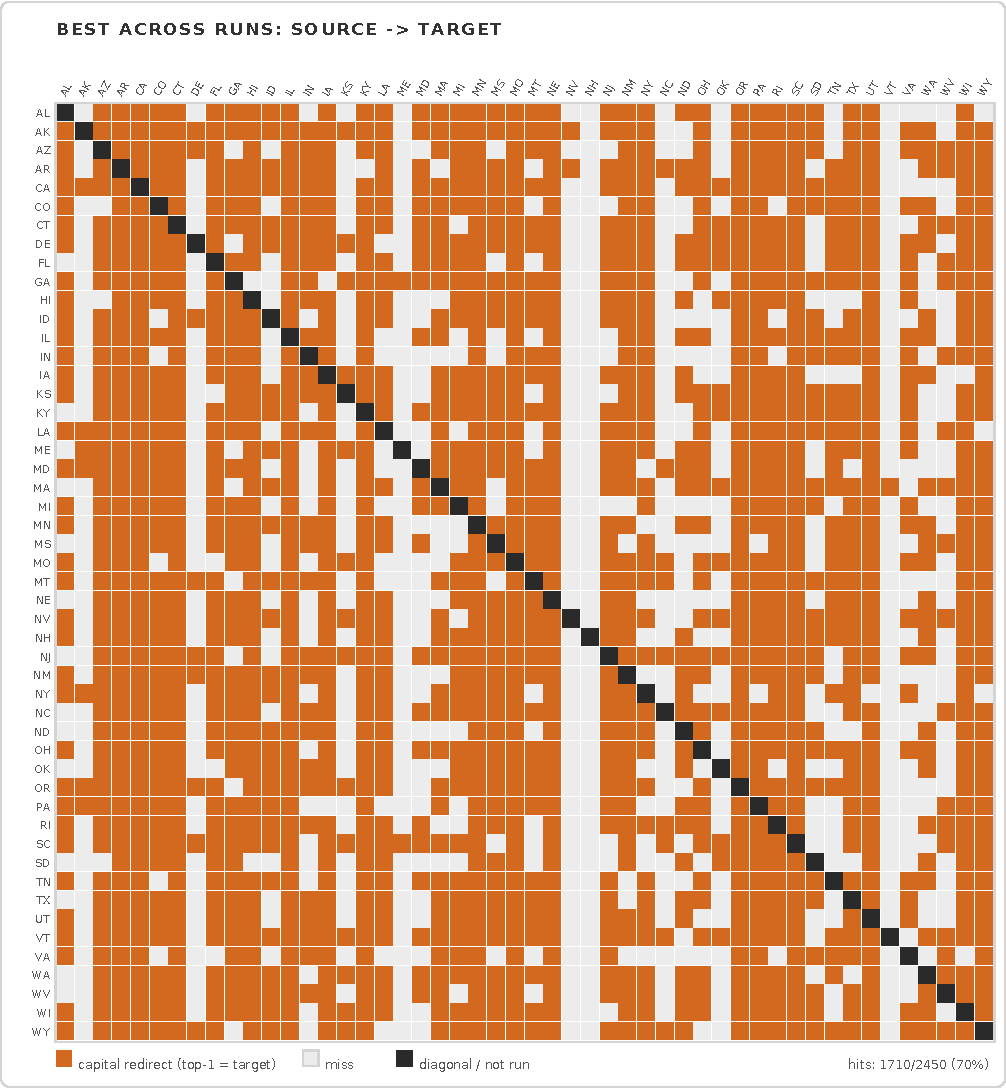
\includegraphics[width=\linewidth]{figures/swap_matrix.pdf}
  \caption{Source $\to$ target swap matrix on the 50-state USA panel
    ($n{=}2{,}450$ pairs, hit-rate $69.8$\%). By default we steer on all
    three concept fields (state + capital + city); each cell additionally
    considers every smaller field subset and reports the winning
    configuration. The winner is the variant that hits the target capital
    (steered top-1 = target capital first-token); when several variants
    hit, we prefer the one that maximises the steered margin of the target
    logit over the next-best capital in the dataset, breaking remaining
    ties by intermediate hit flags and target rank in the baseline logits.
    Cells are coloured by the winning field subset; the 3-field default
    wins only $13$\% of cells, the rest succeed with a strict subset
    (\S\ref{sec:results:diagnostic:fields}). Grey cells: miss; black on
    the diagonal: pair not run.}
  \label{fig:swap-matrix}
\end{figure}

\begin{figure}[!t]
  \centering
  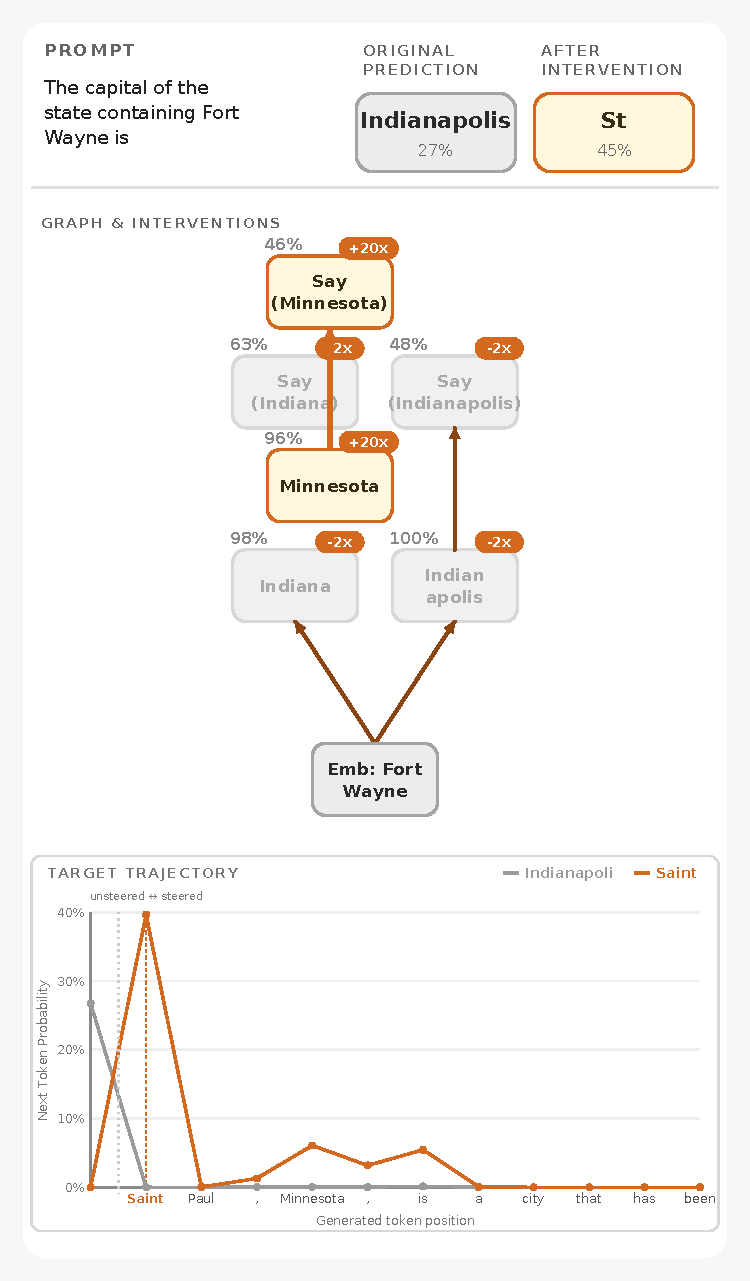
\includegraphics[width=0.85\linewidth]{figures/swap_v2_in_mn.pdf}
  \caption{A representative entity-swap intervention on the USA panel:
    Indiana$\to$Minnesota, probed via ``the state containing Fort Wayne''.
    The top row shows the prompt and the pre/post-intervention prediction
    (\texttt{Indianapolis} $\to$ \texttt{St}, i.e.\ \texttt{Saint~Paul}). The
    middle row shows the labeled supernodes with ablation ($-2\times$) of the
    source state/capital nodes and amplification ($+20\times$) of the target
    state/capital nodes. The bottom row shows the next-token probability sweep
    at $M{=}0$ vs.\ $M{=}20$, with the target trajectory (\texttt{Saint}) rising
    at the steered position while the original (\texttt{Indianapolis}) collapses.}
  \label{fig:swap-examples}
\end{figure}
